\chapter{Boucles}
\introduction{Tant que tu n'y arrives pas recommence.}
On s'intéresse dans ce chapitre aux \textit{structures itératives}, plus communément appelée \textit{boucles}.\\


\section{La boucle while}

Voici son schéma de fonctionnement :
\begin{center}
    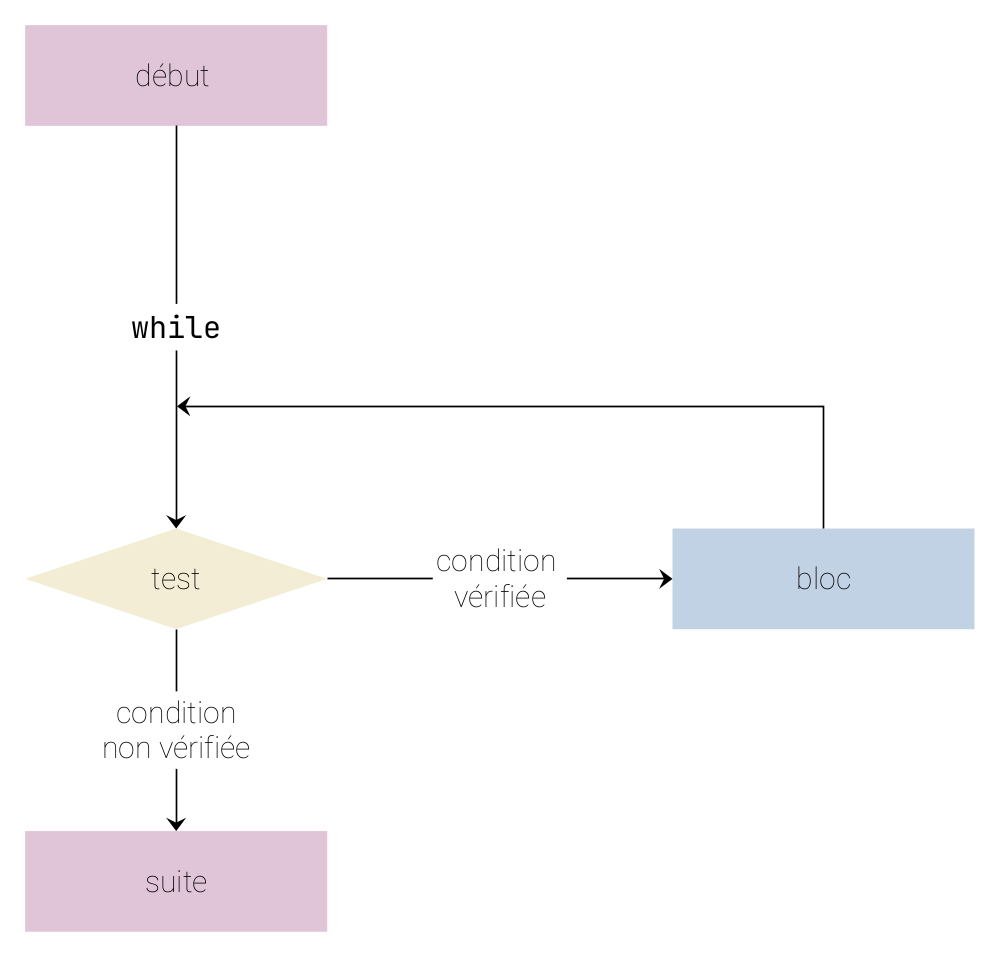
\includegraphics[height=7.5cm]{ch-boucles/img/while.png}
\end{center}

La boucle \mintinline{python}{while} exécute un bloc d'instructions conditionnel \textit{tant que} une condition est vérifiée.\\
Dès que la condition n'est plus vérifiée, le bloc conditionnel n'est plus exécuté.

\begin{pys}
\begin{minted}{python}
reponse=''
print('Bonjour !')
while reponse !='n':
    reponse = input('Voulez-vous continuer ? (o/n) : ')
print('Au revoir.')
\end{minted}
\end{pys}
La boucle \mintinline{python}{while} doit être utilisée avec soin : si la condition est toujours vérifiée, le programme ne s'arrêtera pas :

\begin{pyc}
\begin{minted}{python}
while True:
    print('Au secours !')
\end{minted}
\end{pyc}
Voici un exemple typique d'utilisation de la boucle \mintinline{python}{while} : \\

On place un capital de 2000 euros sur un compte à intérêts annuels de 2\%. On aimerait savoir au bout de combien de temps, sans rien toucher, le 
solde du compte dépassera 2300 euros.\\

\begin{pyc}
\begin{minted}{python}
solde = 2000  # solde initial
n = 0  # nombre d'annees
while solde <= 2300:  # condition de boucle
    n += 1  # augmente le compteur d'annees
    solde *= 1.02  # actualise le solde
print(' Il nous faudra ', n, 'ans.')  # affichage final   
\end{minted}
\end{pyc}

\section{La boucle for ... in range(...)}

Commençons par examiner un nouveau type : \mintinline{python}{range} (plage de valeurs)

\begin{pys}
\begin{minted}{python}
>>> a = range(10)
>>> type(a)
>>> print(list(a))
\end{minted}
\end{pys}

Si \mintinline{python}{range(10)} ressemble beaucoup à la liste \mintinline{python}{[0,1,...,9]}, la finalité de \\\mintinline{python}{range(10)} est d'être un \textit{itérateur}, 
c'est-à-dire une objet dont on peut parcourir le contenu pour créer une boucle :

\begin{pyc}
\begin{minted}{python}
for i in range(10):
    print(i)
\end{minted}
\end{pyc}
La syntaxe complète de \mintinline{python}{range} est : \mintinline{python}{range(<debut>,fin,<increment>)}.\\

Par défaut, si ce n'est pas précisé, \mintinline{python}{debut=0}, et \mintinline{python}{increment=1}.\\

\mintinline{python}{range(<debut>,fin,<increment>)} renvoie la plage de valeurs suivantes :
\begin{itemize}
    \item   On part de la valeur de début, appelons la \mintinline{python}{val}
    \item   Tant que \mintinline{python}{val < fin}:\\
    $\qquad$ - ajouter \mintinline{python}{val} à la plage\\
    $\qquad$ - ajouter \mintinline{python}{increment} à \mintinline{python}{val}
\end{itemize}
Ainsi, \mintinline{python}{range(2,52,10)} renvoie la plage de valeurs \mintinline{python}{2,12,22,32,42}, mais\\ \mintinline{python}{range(2,53,10)} renvoie la plage de valeurs 
\mintinline{python}{2,12,22,32,42,52}.\\

Très souvent, on se contente d'utiliser une instruction du type \mintinline{python}{range(n)}, où \mintinline{python}{n} est de type \mintinline{python}{int}.\\


Voici un exemple : Calculons $1+2+\ldots+100$ :

\begin{pyc}
\begin{minted}{python}
somme = 0
for i in range(1, 101):
    somme += i
print(somme)
\end{minted}
\end{pyc}

\section{La boucle for ... in ...}

On peut généraliser le paragraphe précédent à toute \textit{variable itérable}, c'est extrêmement puissant : les \mintinline{python}{str}, les \mintinline{python}{list} et les 
\mintinline{python}{dict} sont des types itérables.\\

Voici des exemples :\\

Comptons le nombre de voyelles d'une chaîne de caractères :

\begin{pyc}
\begin{minted}{python}
voyelles = 'aeiouy'  # ensemble de voyelles
phrase = input('Entrez une phrases sans accents : ').lower()  # phrase mise en minuscules
compteur = 0  # comptera les voyelles
for lettre in phrase:  # on parcourt la phrase
    if lettre in voyelles:  # est-ce une voyelle ?
        compteur += 1  # si oui on comptabilise
print('Nombre de voyelles : ', compteur)  # affiche le nombre
\end{minted}
\end{pyc}

Faisons la moyenne d'une liste de notes :


\begin{pyc}
\begin{minted}{python}
liste_notes = [12, 11.5, 13, 18, 13, 11, 9]
moyenne = 0
for note in liste_notes:
    moyenne += note
moyenne /= len(liste_notes)
print(moyenne)
\end{minted}
\end{pyc}

Pour le dernier exemple on utilise le type \mintinline{python}{dict} : soit \mintinline{python}{a} une variable de ce type :
\begin{itemize}
    \item   \mintinline{python}{a.keys()} renvoie la liste des clés (des indices du dictionnaire).
    \item   \mintinline{python}{a.values()} renvoie la liste des valeurs prises par le dictionnaire.
\end{itemize}

Voici un second programme de moyenne :

\begin{pyc}
\begin{minted}{python}
resultats = {'EPS': 12, 'maths': 15, 'info': 18}
moyenne = 0
for note in resultats.values():
    moyenne += note
moyenne /= len(resultats)
print(moyenne)
\end{minted}
\end{pyc}

\section{Quelle boucle utiliser ?}

Si la boucle dépend d'une condition particulière on préfèrera la boucle \mintinline{python}{while}.

Si le nombre d'itérations de la boucle est connu on préfèrera une boucle \mintinline{python}{for}.

On peut utiliser une boucle \mintinline{python}{for} sur toute \textit{structure itérative}, par exemple 
    une variable de type \mintinline{python}{range}, \mintinline{python}{str}, \mintinline{python}{list} ou, dans une certaine mesure, \mintinline{python}{dict}.
    
\section{Exercices}
\begin{exercice}
    Calculer à l'aide d'un script la somme des carrés des 1000 premiers entiers non nuls.
\end{exercice}

%----------------------------------------------------------------------
\begin{exercice}
    Calculer à l'aide d'un script la somme des carrés des 1000 premiers multiples de 3 non nuls.
\end{exercice}

%---------------------------------------------------------------------
\begin{exercice}
    \'Ecrire un script qui demande une phrase à l'utilisateur, puis affiche la phrase en rajoutant des tirets.\\
    Exemple : on entre \mintinline{python}{'Salut à toi'} le script affiche \mintinline{python}{'S-a-l-u-t- -à- -t-o-i-}.
\end{exercice}

\begin{exercice}
    Calculer à l'aide d'un script le nombre $n$ à partir duquel la somme $1^2+2^2+\ldots+n^2$ dépasse un milliard.
\end{exercice}

%----------------------------------------------------------------------
\begin{exercice}
    \'Ecrire un script qui demande une phrase et compte le nombre d'occurrences de la lettre \og a \fg{} dans celle-ci.
\end{exercice}

%----------------------------------------------------------------------
\begin{exercice}
    Programmer le jeu du "plus petit plus grand" :
    \begin{itemize}
        \item   L'ordinateur choisit un nombre entier au hasard compris entre 0 et 100.\\
        Au début du script, importer la fonction \mintinline{python}{randint} du module \mintinline{python}{random} avec \mintinline{python}{form random import randint}.\\
        Pour obtenir un entier au hasard, utiliser \mintinline{python}{randint(0,100)}.
        \item   L'utilisateur propose un nombre, l'ordinateur répond \og gagné\fg, \og plus petit\fg{} ou \og plus grand\fg.
        \item   Le programme continue tant que l'utilisateur n'a pas gagné.
    \end{itemize}
\end{exercice}

%----------------------------------------------------------------------
\begin{exercice}
    On considère la suite $s$ définie par:
    \tabulardefault
    $$\left\{
    \begin{array}{llll}
    s_0 & = & 1000 & \\
    s_{n+1} & = & 0,99s_n+1 & \textrm{pour tout } n\in\mathbf{N}
    \end{array}
    \right. $$
    
    \begin{itemize}
        \item   \'Ecrire un script calculant les premiers termes de $s$ (vous décidez le nombre de termes).
        \item   Utiliser ce script pour conjecturer la limite de $s$.
        \item   Modifier ce script pour obtenir le plus petit entier $n$ tel que l'écart entre $s_n$ et sa limite soit inférieur ou égal à $10^{-4}$.
        
    \end{itemize}
\end{exercice}

%----------------------------------------------------------------------
\begin{exercice}
    $\varphi$ (lettre phi, équivalent du \og f \fg{} en grec) est défini par : $$\varphi=1+\frac{1}{1+\frac{1}{1+\frac{1}{\ldots}}}$$
    Sur papier, fabriquer une suite par récurrence commençant ainsi :
    \begin{itemize}
        \item   1
        \item   $1+\frac{1}{1}$
        \item   $1+\frac{1}{1+\frac{1}{1}}$
        \item   Et c\ae tera (trouver une relation simple pour calculer le terme suivant à partir du terme actuel).
    \end{itemize}
    Programmer un script qui calcule successivement les termes de cette suite (aller jusqu'à 10000\eme).\\
    
    Comparer avec la valeur exacte de $\varphi$, qui est $\frac{1+\sqrt{5}}{2}$.
\end{exercice}

\begin{exercice}
    \'Ecrire un script qui détermine si un entier est premier ou pas.
\end{exercice}